%%%%%%%%%%%%%%%%%%%%%%%%%%%%%%%%%%%%%%%%%%%%%%%%%%%%%%%%%%%%%%%%%%%%%%%%%%%%%%%%
%%%%%%%%%%%%%%%%%%   Vorlage für eine Abschlussarbeit   %%%%%%%%%%%%%%%%%%%%%%%%
%%%%%%%%%%%%%%%%%%%%%%%%%%%%%%%%%%%%%%%%%%%%%%%%%%%%%%%%%%%%%%%%%%%%%%%%%%%%%%%%

% Erstellt von Maximilian Nöthe, <maximilian.noethe@tu-dortmund.de>
% ausgelegt für lualatex und Biblatex mit biber

% Kompilieren mit
% lualatex dateiname.tex
% biber dateiname.bcf
% lualatex dateiname.tex
% lualatex dateiname.tex
% oder einfach mit:
% make

\documentclass[
  tucolor,
  BCOR=12mm,     % 12mm binding corrections, adjust to fit your binding
  parskip=half,  % new paragraphs start with half line vertical space
  open=any,      % chapters start on both odd and even pages
  cleardoublepage=plain,  % no header/footer on blank pages
]{tudothesis}


% Warning, if another latex run is needed
\usepackage[aux]{rerunfilecheck}

% just list chapters and sections in the toc, not subsections or smaller
\setcounter{tocdepth}{1}

%------------------------------------------------------------------------------
%------------------------------ Sprache und Schrift: --------------------------
%------------------------------------------------------------------------------
\usepackage{fontspec}
\defaultfontfeatures{Ligatures=TeX}  % -- becomes en-dash etc.

% german language
\usepackage{polyglossia}
\setdefaultlanguage{german}

% for english abstract and english titles in the toc
\setotherlanguages{english}

% intelligent quotation marks, language and nesting sensitive
\usepackage[autostyle]{csquotes}

% microtypographical features, makes the text look nicer on the small scale
\usepackage{microtype}

%------------------------------------------------------------------------------
%------------------------ Für die Matheumgebung--------------------------------
%------------------------------------------------------------------------------

\usepackage{amsmath}
\usepackage{amssymb}
\usepackage{mathtools}

% Enable Unicode-Math and follow the ISO-Standards for typesetting math
\usepackage[
  math-style=ISO,
  bold-style=ISO,
  sans-style=italic,
  nabla=upright,
  partial=upright,
]{unicode-math}
\setmathfont{Latin Modern Math}

% nice, small fracs for the text with \sfrac{}{}
\usepackage{xfrac}


%------------------------------------------------------------------------------
%---------------------------- Numbers and Units -------------------------------
%------------------------------------------------------------------------------

\usepackage[
  locale=DE,
  separate-uncertainty=true,
  per-mode=symbol-or-fraction,
]{siunitx}
\sisetup{math-micro=\text{µ},text-micro=µ}

%------------------------------------------------------------------------------
%-------------------------------- tables  -------------------------------------
%------------------------------------------------------------------------------

\usepackage{booktabs}       % stellt \toprule, \midrule, \bottomrule

%------------------------------------------------------------------------------
%-------------------------------- graphics -------------------------------------
%------------------------------------------------------------------------------

\usepackage{graphicx}
\usepackage{grffile}

% allow figures to be placed in the running text by default:
\usepackage{scrhack}
\usepackage{float}
\floatplacement{figure}{htbp}
\floatplacement{table}{htbp}

% keep figures and tables in the section
\usepackage[section, below]{placeins}


%------------------------------------------------------------------------------
%---------------------- customize list environments ---------------------------
%------------------------------------------------------------------------------

\usepackage{enumitem}

%------------------------------------------------------------------------------
%------------------------------ Bibliographie ---------------------------------
%------------------------------------------------------------------------------

\usepackage[
  backend=biber,   % use modern biber backend
  autolang=hyphen, % load hyphenation rules for if language of bibentry is not
                   % german, has to be loaded with \setotherlanguages
                   % in the references.bib use langid={en} for english sources
]{biblatex}
\addbibresource{references.bib}  % die Bibliographie einbinden
\DefineBibliographyStrings{german}{andothers = {{et\,al\adddot}}}

%------------------------------------------------------------------------------
%------------------------------ Sonstiges: ------------------------------------
%------------------------------------------------------------------------------

\usepackage[pdfusetitle,unicode,linkbordercolor=tugreen]{hyperref}
\usepackage{bookmark}
\usepackage[shortcuts]{extdash}

\usepackage{tikz-feynman}
\usepackage{todonotes}

\DeclarePairedDelimiter{\bra}{\langle \,}{\, \lvert}
\DeclarePairedDelimiter{\ket}{\lvert \, }{\, \rangle}
\DeclarePairedDelimiterX{\braket}[2]{\langle}{\rangle}{
  #1 \delimsize| #2
}

%------------------------------------------------------------------------------
%-------------------------    Angaben zur Arbeit   ----------------------------
%------------------------------------------------------------------------------

\author{Jean-Marco Alameddine}
\title{Theoretische Untersuchung von Formfaktoren in \texorpdfstring{$B \to D l \overline \nu_l$}{B -> D l nu_l}}
\date{2017}
\birthplace{Iserlohn}
\chair{Lehrstuhl für Theoretische Physik III}
\division{Fakultät Physik}
\thesisclass{Bachelor of Science}
\submissiondate{21. Juli 2017}
\firstcorrector{Prof.~Dr.~Gudrun Hiller}
\secondcorrector{Prof.~Dr.~Zweitgutachter}

% tu logo on top of the titlepage
\titlehead{\includegraphics[height=1.5cm]{logos/tu-logo.pdf}}

\begin{document}
\frontmatter
%\thispagestyle{empty}
\setcounter{page}{2}
\section*{Hinweise}
Empfohlen wird die Verwendung dieser Vorlage mit der jeweils aktuellsten TeXLive Version (Linux, Windows) bzw. MacTeX Version (MacOS).
Aktuell ist dies TeXLive 2016. Download hier:
\begin{center}
  \ttfamily\url{https://www.tug.org/texlive/}
\end{center}
Bei Verwendung von TexLive Versionen 2014 und älter sollte
die Zeile
\begin{center}
\verb+\RequirePackage{fixltx2e}+ 
\end{center}
als erste Zeile der Präambel noch vor der Dokumentenklasse eingefügt werden.
Dies lädt diverse Bugfixes für LaTeX, die ab TexLive 2015 Standard sind.

Die Vorlage \texttt{thesis.tex} ist für die Kompilierung mit \texttt{lualatex} ausgelegt, mit wenigen Anpassungen kann sie aber auch mit \texttt{pdflatex} oder \texttt{xelatex} verwendet werden. 
Die Dokumentenklasse \texttt{tudothesis.cls} kann mit allen drei Programmen verwednet werden.

Achten Sie auch auf die Kodierung der Quelldateien.
Bei Verwendung von Xe\LaTeX\ oder Lua\LaTeX\ (empfohlen) müssen die
Quelldateien UTF-8 kodiert sein.
Bei Verwendung von pdf\LaTeX\ nutzen Sie die Pakete \texttt{inputenc} und \texttt{fontenc} mit der korrekten Wahl der Kodierungen.

Eine aktuelle Version dieser Vorlage steht unter 
\begin{center}
  \ttfamily\url{https://github.com/maxnoe/tudothesis}
\end{center}
zur Verfügung.

Alle verwendeten Pakete werden im \LaTeX{} Kurs von Pep et al.\ erklärt:
\begin{center}
  \ttfamily\url{http://toolbox.pep-dortmund.org/notes}
\end{center}

Für Rückmeldungen und bei Problemen mit der Klasse oder Vorlage, bitte ein \emph{Issue} auf GitHub aufmachen oder eine Email an
\href{mailto:maximilian.noethe@tu-dortmund.de}{maximilian.noethe@tu-dortmund.de} schreiben.

Wenn Sie die Dokumentenklasse mit der Option \texttt{tucolor} laden, werden verschiedene Elemente in TU-Grün gesetzt.

\maketitle

% Gutachterseite
\makecorrectorpage

% hier beginnt der Vorspann, nummeriert in römischen Zahlen
\thispagestyle{plain}

\section*{Kurzfassung}
In dieser Arbeit wird der semileptonische Zerfall $\overline{B} \to D l \overline{\nu}_l$ untersucht.
Dabei werden die Formfaktoren $f_+(z)$, $f_0(z)$ des Zerfalles durch Fitten an Gittereichrechnungen einer vorliegenden Arbeit ermittelt.
Hierbei wird als Fitfunktion die \enquote{Simplified Series Expansion} mit verschiedenen Ordnungen der Reihenentwicklung verwendet.
Aus den Formfaktoren wird die differentielle Zerfallsbreite des Zerfalles und hieraus die Observable $R(D)$ zu $R(D) = \SI{0.288+-0.011}{}
$ bestimmt, wobei sich eine Abweichung von $\SI{2.4}{}
\sigma$ zu den experimentellen Werten von Belle und BaBar ergibt.
Diese mögliche Diskrepanz wird zuerst durch die Anpassung der Formfaktoren im Standardmodell und danach durch die Einführung einer neuen Kopplung im Tauonen-Sektor, beschrieben durch den Wilsonkoeffizienten $C_{\text{S}1}$, behoben.
Es wird der mögliche Parameterbereich von $C_{\text{S}1}$, damit $R(D)$ mit den experimentellen Werten übereinstimmt, angegeben.


\section*{Abstract}
\begin{english}
This thesis examines the semileptonic decay $\overline{B} \to D l \overline{\nu}_l$.
Using lattice calculations from an existent paper, the relevant form factors $f_+(z)$, $f_0(z)$ are determined by fitting to these data.
As a fit function, the \enquote{Simplified Series expansion} is used, considering several expansion orders.
The differential decay rate as well as the observable $R(D)$ follow from the results for the form factors.
The calculated result $R(D) = \SI{0.288+-0.011}{}
$ portrays an $\SI{2.4}{}
\sigma$ deviation from the experimental results reported by Belle and BaBar.
This possible disagreement is treated by altering the form factors within the Standard Model as well as introducing a BSM coupling, affecting the tau lepton decay rate only, which is described by the Wilson Coefficient $C_{\text{S}1}$.
The regions for $C_{\text{S}1}$ to conform with the experimental data of $R(D)$ are presented.
\end{english}

\tableofcontents

\mainmatter
% Hier beginnt der Inhalt mit Seite 1 in arabischen Ziffern
\chapter{Einleitung}

Das Standardmodell der Elementarteilchenphysik beschreibt den Aufbau der Materie mit einer beeindruckenden Genauigkeit.
Es führt die Zusammensetzung der Materie auf die Elementarteilchen Quarks, Leptonen, Eichbosonen sowie das Higgs-Boson zurück.
Als Wechselwirkungen existieren die elektromagnetische Wechselwirkung, die starke Wechselwirkung, die schwache Wechselwirkung sowie die Gravitation, wobei letztere durch die allgemeine Relativitätstheorie beschrieben werden muss.
Aufgrund des großen Erfolges des Standardmodells ist es umso interessanter, Beobachtungen zu finden, welche nicht mit der aktuellen Theorie übereinstimmen oder nicht durch diese beschrieben werden.
Hierzu gehören beispielsweise Neutrinooszillationen oder die Asymmetrie zwischen Materie und Antimaterie im Universum.
All diese Erscheinungen bilden die Grundlage für die Einführung neuer Physik außerhalb des Standardmodells.

Ein Hinweis auf neue Physik durch eine solche Diskrepanz, welche in dieser Arbeit untersucht werden soll, findet sich in semileptonischen Zerfällen von $B$-Mesonen in $D$-Mesonen.
Für diesen Zerfall existieren experimentelle Messungen der Observable $R(D)$, welche jedoch von den theoretischen Berechnungen signifikant abweichen.
Fundamental für die theoretische Beschreibung dieses Zerfalles sind die sogenannten Formfaktoren, welche in dieser Arbeit mit besonderen Blick auf die Observable $R(D)$ untersucht werden sollen.

Zunächst wird in Kapitel \ref{sec:theorie} eine theoretische Beschreibung des zugrunde liegenden Zerfalles sowie in diesem Zusammenhang eine Definition der verwendeten Formfaktoren angegeben.
Zusätzlich werden die Kinematik des Zerfalles und die möglichen Parametrisierungen des auftretenden Impulsübertrages kurz beschrieben.
Daraufhin werden in Kapitel \ref{make} die Formfaktoren anhand von Gittereichrechnungen für diskrete Impulsüberträge aus \cite{PhysRevD.92.034506} bestimmt.
Hierzu wird zunächst die verwendete Fitmethodik erläutert und der Fit für verschiedene Reihenentwicklungen als Fitfunktionen durchgeführt.
Daraufhin werden die differenziellen Zerfallsbreiten sowie die Observable $R(D)$ aus den ermittelten Fitergebnissen bestimmt.
Abschließend werden Korrekturen der Formfaktoren sowie mögliche Einflüsse durch neue Physik außerhalb des Standardmodells einbezogen, um eine mögliche Erklärung für die Diskrepanz zu den experimentellen Daten bereitzustellen.

\chapter{Theorie des semileptonischen Zerfalles}

\section{Qualitative Beschreibung}

Das Feynman-Diagramm in führender Ordnung des untersuchten Zerfalles ist in Abbildung \ref{fig:feynman1} dargestellt.

\todo{Sich für den schönsten Feynmangraphen entscheiden}
\begin{figure}
  \centering
  \begin{tikzpicture}
  \begin{feynman}
    \vertex (a1) {\(b\)};
    \vertex[right=1cm of a1] (a2);
    \vertex[right=1cm of a2] (a3);
    %\vertex[right=1cm of a3] (a4) {\(b\)};
    \vertex[right=1cm of a3, label=125:\(V_{cb}\)] (a5);
    \vertex[right=2cm of a5] (a6) {\(c\)};

    \vertex[below=2em of a1] (b1) {\(\overline q\)};
    \vertex[right=1cm of b1] (b2);
    \vertex[right=1cm of b2] (b3);
    %\vertex[right=1cm of b3] (b4) {\(\overline d\)};
    \vertex[below=2em of a6] (b5) {\(\overline q\)};

    \vertex[above=of a6] (c1) {\(\overline \nu_l\)};
    \vertex[above=2em of c1] (c3) {\(l\)};
    \vertex at ($(c1)!0.5!(c3) - (1cm, 0)$) (c2);

    \diagram* {
      {[edges=fermion]
        (b5) -- (b1)
        (a1) -- (a5) -- (a6)
        %(b5) -- (b4) -- (b3) -- (a3) -- (a4) -- (a5) -- (a6),
      },


      (c1) -- [fermion, out=180, in=-45] (c2) -- [fermion, out=45, in=180] (c3),
      (a5) -- [boson, edge label=\(W^{-}\)] (c2),
    };

    \draw [decoration={brace}, decorate] (b1.south west) -- (a1.north west)
          node [pos=0.5, left] {\(\overline B\)};
    %\draw [decoration={brace}, decorate] (c3.north east) -- (c1.south east)
    %      node [pos=0.5, right] {\(\pi^{-}\)};
    \draw [decoration={brace}, decorate] (a6.north east) -- (b5.south east)
          node [pos=0.5, right] {\(D\)};
  \end{feynman}
  \end{tikzpicture}
  \caption{Feynman-Diagramm des semileptonischen Zerfalles $B \to D l \overline \nu_l$ in führender Ordnung.}
  \label{fig:feynman1}
\end{figure}

Im Eingangszustand befindet sich ein $\overline B$-Meson, welches aus einem $b$-Quark und einem leichten Antiquark $\overline q$ ($ \overline q = \overline u, \overline d)$ besteht.
Die schwache Wechselwirkung führt zu einer Umwandlung des beteiligten $b$-Quarks in ein $c$-Quark unter Emission eines $W^{-}$-Bosons. Dieses $W^{-}$-Boson ist ein virtuelles Teilchen und zerfällt direkt weiter in ein Lepton $l$ und das dazugehörige Antineutrino $\overline \nu_l$.
Zusätzlich ist bei diesem Prozess zu beachten, dass die schwache Wechselwirkung nicht an die Masseneigenzustände der Quarks koppelt.
Die korrekten Eigenzustände der Quarks $d'$, $s'$ und $b'$ für die schwache Wechselwirkung sind stattdessen Linearkombinationen der Masseneigenzustände von $d$, $s$ und $b$. Sie ergeben sich somit durch eine Rotation der ursprünglichen Eigenzustände.
Diese Rotation wird durch die unitäre CKM-Matrix beschrieben.
Der für den betrachteten Zerfall relevante Parameter $\lvert V_{cb} \rvert$ beträgt \cite{Bigi2017441}
\begin{equation}
  \lvert V_{cb} \rvert = \SI{40.49+-0.97e-3}{}
.
\end{equation}

\begin{figure}
  \centering
  \begin{tikzpicture}
  \begin{feynman}
    \vertex (a1) {\(b\)};
    \vertex[right=1cm of a1] (a2);
    \vertex[right=1cm of a2] (a3);
    %\vertex[right=1cm of a3] (a4) {\(b\)};
    \vertex[right=1cm of a3, label=125:\(V_{cb}\)] (a5);
    \vertex[right=2cm of a5] (a6) {\(c\)};

    \vertex[below=4em of a1] (b1) {\(\overline q\)};
    \vertex[right=1cm of b1] (b2);
    \vertex[right=1cm of b2] (b3);
    \vertex[below=2em of a3] (g1);
    \vertex[left=1.8cm of a6] (g2);
    \vertex[right=1cm of b2] (g5);
    \vertex[left=0.5cm of a6] (g6);
    \vertex[right=1.5cm of g1] (g3);
    \vertex[right=0.8cm of g3] (g4);
    %\vertex[right=1cm of b3] (b4) {\(\overline d\)};
    \vertex[below=4em of a6] (b5) {\(\overline q\)};

    \vertex[above=of a6] (c1) {\(\overline \nu_l\)};
    \vertex[above=2em of c1] (c3) {\(l\)};
    \vertex at ($(c1)!0.5!(c3) - (1cm, 0)$) (c2);

    \diagram* {
      {[edges=fermion]
        (b5) -- (b1)
        (a1) -- (a5) -- (a6)
        %(b5) -- (b4) -- (b3) -- (a3) -- (a4) -- (a5) -- (a6),
      },


      (c1) -- [fermion, out=180, in=-45] (c2) -- [fermion, out=45, in=180] (c3),
      (a5) -- [boson, edge label=\(W^{-}\)] (c2),

      (a2) -- [gluon] (g1)
      (b2) -- [gluon] (g1)
      (g1) -- [gluon] (g2)
      (g5) -- [gluon] (g3)
      (g3) -- [fermion, half left] (g4)
      (g4) -- [fermion, half left] (g3)
      (g4) -- [gluon] (g6)

    };

    \draw [decoration={brace}, decorate] (b1.south west) -- (a1.north west)
          node [pos=0.5, left] {\(\overline B\)};
    %\draw [decoration={brace}, decorate] (c3.north east) -- (c1.south east)
    %      node [pos=0.5, right] {\(\pi^{-}\)};
    \draw [decoration={brace}, decorate] (a6.north east) -- (b5.south east)
          node [pos=0.5, right] {\(D\)};
  \end{feynman}
  \end{tikzpicture}
  \caption{Exemplarisches Feynman-Diagramm des semileptonischen Zerfalles $B \to D l \overline \nu_l$ unter Berücksichtigung der starken Wechselwirkung zwischen den beteiligten Quarks.}
  \label{fig:feynman2}
\end{figure}

Zusätzlich ist bei der Beschreibung des vorliegenden Zerfalles die starke Wechselwirkung zu berücksichtigen.
Sie führt, vermittelt durch den Austausch von Gluonen, zur Bindung zwischen dem als Zuschauerquark agierenden Antiquark sowie dem schwach wechselwirkenden Quark.
Aufgrund des nicht-pertubativen Verhaltens der starken Wechselwirkung bei großen Abständen werden auch die Beiträge der Feynman-Diagramme höherer Ordnung, wie in Abbildung \ref{fig:feynman2} exemplarisch dargestellt, relevant.
Primäres Ziel der Formfaktoren ist es, diese Effekte bei der Berechnung der Zerfallsraten quantitativ zu Berücksichtigen.

\section{Parametrisierung des Matrixelementes durch Formfaktoren}

Das Matrixelement $M$ des Zerfalles lässt sich allgemein als \todo{Abstände zwischen den Bra/Kets optimieren}
\begin{align*}
  M = \bra{D \, l \, \overline{\nu_l}} H \ket{ \overline{B} }
\end{align*}
mit dem Hamiltonian $H$ des Zerfalles beschreiben.
Es ist außerdem möglich, das Matrixelement in einen hadronischen Anteil mit dem Hamiltonian $H_\text{had}$ und einen leptonischen Anteil mit dem Hamiltonian $H_\text{lep}$ zu faktorisieren, so dass sich das Matrixelement
\begin{align*}
  M = \bra{ l \, \overline{\nu_l}} H_\text{lep} \ket{0}  \bra{D} H_\text{had}  \ket{ \overline{B} }
\end{align*}
ergibt.
Der hadronische Faktor wird durch einen V-A-Strom
\begin{align*}
  \bra{D} H_\text{had}  \ket{ \overline{B} } = \bra{D} \, \overline{c} \gamma_\mu (1 - \gamma_5) b \, \ket{ \overline{B} } = \bra{D} \underbrace{\overline{c} \gamma_\mu b }_{= V_\mu} \ket{\overline{B} } - \bra{D} \, \underbrace{ \overline{c} \gamma_\mu \gamma_5 b}_{= A_\mu}\, \ket{ \overline{B} }
\end{align*}
beschrieben, wobei $b$ hier der Spinor des $b$-Quarks und $\overline{c}$ der adjungierte Spinor des $c$-Quarks ist.
Die Bezeichnungen $V_\mu$ und $A_\mu$ für die Ströme drücken aus, dass sich unter Parität $V_\mu = \overline{c} \gamma_\mu b$ wie ein Vektor und $A_\mu = \overline{c} \gamma_\mu \gamma_5 b$ wie ein Axialvektor transformiert.
Da die hier betrachteten Mesonen pseudoskalare Größen sind, stehen zur Parametrisierung des Matrixelementes als dynamische Variablen der Viererimpuls des $\overline{B}$-Mesons $p^B$ sowie der Viererimpuls des $D$-Mesons $p^D$ zur Verfügung.
Zusätzlich lässt sich hieraus der Lorentz-Skalar
\begin{equation}
  q^2 = (p^B-p^D)^2
\end{equation}
konstruieren, welcher den Impulsübertrag zwischen den Mesonen ausdrückt.

Sowohl die dynamische Variable $p^B$ als auch $p^D$ transformieren sich wie Vektoren.
Aus diesen Größen lässt sich jedoch kein Ausdruck konstruieren, der sich wie ein Axialvektor transformiert.
Da die Quantenchromodynamik die Parität erhält, folgt hieraus direkt, dass der axiale Anteil des hadonischen Matrixelementes verschwinden muss:
\begin{align*}
  \bra{D} A_\mu \ket{\overline{B}} = 0.
\end{align*}
Somit verbleibt der vektorielle Anteil des hadronischen Matrixelementes, welcher durch
\begin{equation}
  \bra{D} V_\mu \ket{\overline{B}} = f_+(q^2)(p^B + p^D)_\mu + f_{-}(q^2)(p^B - p^D)_\mu
\end{equation}
mit den Formfaktoren $f_+(q^2)$, $f_{-}(q^2)$ parametrisiert wird.

Mithilfe dieser Parametrisierung kann, unter Nutzung der Feynmanregeln, die differentielle Zerfallsbreite für den betrachteten Zerfall berechnet werden.
Sie ergibt sich zu \cite{PhysRevD.94.094008}
\begin{equation}
  \frac{\mathrm{d} \Gamma}{\mathrm{d} q^2} \left(\overline{B} \to D l \overline{\nu_l} \right) = \frac{\eta_\text{EW}^2 G_\text{F}^2 \lvert V_{cb} \rvert^2 m_B \sqrt{\lambda} }{192 \pi^3} \left( 1 - \frac{m_l^2}{q^2} \right)^2 \left( c_+^l f_+(q^2)^2 + c_0^l f_0(q^2)^2 \right)
\end{equation}
mit den Abkürzungen
\begin{align*}
  c_+^l &= \frac{\lambda}{m_B^4} \left( 1 + \frac{m_l^2}{2 q^2} \right) & c_0^l &= \left(1 - \frac{m_D^2}{m_B^2} \right)^2 \frac{3 m_l^2}{2 q^2}
\end{align*}
sowie
\begin{align*}
  \lambda = (q^2 - m_B^2 - m_D^2)^2 - 4 m_B^2 m_D^2
\end{align*}
und
\begin{align*}
  f_0(q^2) = f_+(q^2) + f_{-}(q^2) \frac{q^2}{m_B^2 - m_D^2}.
\end{align*}

\section{Kinematik des Zerfalles}

Aus der Viererimpulserhaltung $p^B = p^D + p^l + p^{\overline{\nu_l}}$ lassen sich Einschränkungen an den kinematisch erlaubten Bereich des Impulsübertrages $q^2$ stellen.
Diese Einschränkungen ergeben sich, wenn die beiden kinematischen Extremfälle betrachtet werden, welche jeweils in Abbildung \ref{fig:recoil} skizziert sind.
Es ergibt sich hieraus, dass der Impulsübertrag im Bereich
\begin{equation}
  m_l^2 \leq q^2 \leq (m_B - m_D)^2
  \label{eqn:kinematik}
\end{equation}
liegen kann.
\begin{figure}
  \centering
  \begin{subfigure}{0.48\textwidth}
    \centering
    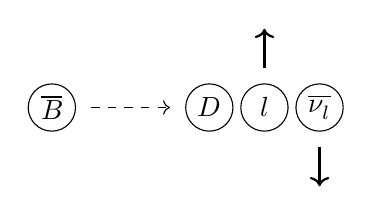
\begin{tikzpicture}
      \draw (0,0) circle [radius=0.3] node {$\overline{B}$};
      \draw[dashed, ->] (0.5, 0) -- (1.5, 0);
      \draw (2,0) circle [radius=0.3] node {$D$};
      \draw (2.7,0) circle [radius=0.3] node {$l$};
      \draw[thick, ->] (2.7, 0.5) -- (2.7, 1.0);
      \draw (3.4,0) circle [radius=0.3] node {$\overline{\nu_l}$};
      \draw[thick, ->] (3.4, -0.5) -- (3.4, -1.0);
    \end{tikzpicture}
    \caption{Kinematik bei $q_\text{max}^2 = (m_B - m_D)^2$.}
    \label{fig:recoil1}
  \end{subfigure}
  \begin{subfigure}{0.48\textwidth}
    \centering
    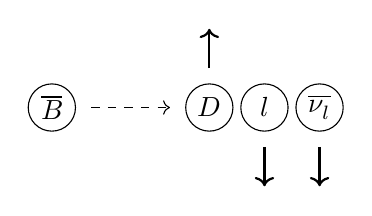
\begin{tikzpicture}
      \draw (0,0) circle [radius=0.3] node {$\overline{B}$};
      \draw[dashed, ->] (0.5, 0) -- (1.5, 0);
      \draw (2,0) circle [radius=0.3] node {$D$};
      \draw[thick, ->] (2, 0.5) -- (2, 1.0);
      \draw (2.7,0) circle [radius=0.3] node {$l$};
      \draw[thick, ->] (2.7, -0.5) -- (2.7, -1.0);
      \draw (3.4,0) circle [radius=0.3] node {$\overline{\nu_l}$};
      \draw[thick, ->] (3.4, -0.5) -- (3.4, -1.0);
    \end{tikzpicture}
    \caption{Kinematik bei $q_\text{min}^2 = m_l^2$.}
    \label{fig:recoil2}
  \end{subfigure}
  \caption{Kinematische Extremfälle beim Impulsübertrag.}
  \label{fig:recoil}
\end{figure}
\todo{Wirklich dieses Diagramm behalten? Und "zero-recoil"-Begriff bei a) einbringen?}

Für den Impulsübertrag $q^2$ werden häufig alternative Parametrisierungen verwendet.
Eine Möglichkeit stellt die $w$-Parametrisierung
\begin{equation}
  w(q^2) = \frac{m_B^2 + m_D^2 - q^2}{2 m_B m_D}
\end{equation}
dar. %, dessen Abhängigkeit von $q^2$ in Abbildung \ref{fig:w_param} dargestellt ist.
Hierbei wird der maximale Impulsübertrag $q_\text{max}^2$ auf $w=0$ abgebildet.

Eine weitere Parametrisierung, welche für den im folgenden Kapitel durchgeführten Fit der Formfaktoren von Bedeutung ist, findet sich in der Variable
\begin{equation}
  z(q^2) = \frac{\sqrt{w+1}-\sqrt{2}}{\sqrt{w+1}+\sqrt{2}}.
\end{equation}
Diese Parametrisierung von $q^2$ bildet den maximalen Impulsübertrag $q_\text{max}^2$ auf $z=0$ ab. %, wie in Abbildung \ref{fig:z_param} dargestellt ist.
Betrachtet man $z(q^2)$ zusätzlich außerhalb des kinematisch erlaubten Bereiches, so wird der Impulsübertrag, wie in Abbildung \ref{fig:z_kreis} dargestellt, auf die komplexe Ebene abgebildet.
Dabei bewegt sich $z$ auf einem Einheitshalbkreis in der oberen komplexen Halbebene, so dass $\lvert z \rvert \leq \num{1}$ immer erfüllt ist.
\begin{figure}
  \centering
  \includegraphics[width=0.9\textwidth]{pycode/plot_z_2.pdf}
  \caption{Abbildung von $q^2$ durch $z$ auf die komplexe Ebene. In grün wird der nach Gleichung \eqref{eqn:kinematik} kinematisch erlaubte Bereich dargestellt. Die gestrichelte rote Line verdeutlicht den unphysikalischen Bereich negativer Impulsüberträge.}
  \label{fig:z_kreis}
\end{figure}

\chapter{Fitten der Formfaktoren innerhalb und außerhalb des Standardmodelles}\label{make}
Das Paper \cite{PhysRevD.92.034506} stellt Theoriewerte für die Formfaktoren $f_+(w)$ und $f_0(w)$ für verschiedene Impulsüberträge $w$ zur Verfügung, welche aus Gittereichrechnungen für den exklusiven Zerfall $\overline{B} \to D l \overline{\nu_l}$ stammen.
Die Berechnungen sind dabei \enquote{unquenched}\todo{Übersetzung für unquenched}, berücksichtigen dementsprechend die Dynamik von involvierten Seequarks.
Die Gittereichrechnungen werden unter Verwendung von 14 verschiedenen Konfigurationen, d.h. Kombinationen von Gitterabständen und Massenverhältnissen von leichten Seequarks und Strange-Seequarks, durchgeführt. \todo{Korrektheit und Vollständigkeit der Sachinhalte?}
In Tabelle \ref{tab:data} sind die dem Paper entnommenen Daten und ihre Fehler, sowie in Abbildung \ref{fig:cor_daten} die Korrelationen der Daten untereinander angegeben.
Alle folgenden Berechnungen werden unter Verwendung dieser Werte durchgeführt.

\begin{figure}
  \centering
  \includegraphics[width=0.8\textwidth]{pycode/cormatrix_daten.pdf}
  \caption{Korrelationsmatrix der Daten der Gittereichrechnungen.}
  \label{fig:cor_daten}
\end{figure}

\begin{table}
  \centering
  \caption{Werte der Formfaktoren aus Gittereichrechnungen für verschiedene Impulsüberträge.}
  \label{tab:data}
  \sisetup{table-format=1.2}
  \begin{tabular}{
    S[table-format=1.2]
    S[table-format=1.4]
    @{${}\pm{}$}
    S[table-format=1.4]
    S[table-format=1.4]
    @{${}\pm{}$}
    S[table-format=1.4]
  }
  \toprule
  {$w$} & \multicolumn{2}{c}{$f_+(w)$} & \multicolumn{2}{c}{$f_0(w)$} \\
  \midrule
  1 & 1.1994 & 0.0095 & 0.9026 & 0.0072 \\
  1.08 & 1.0941 & 0.0104 & 0.8609 & 0.0077 \\
  1.16 & 1.0047 & 0.0123 & 0.8254 & 0.0094 \\
  \bottomrule
  \end{tabular}
\end{table}




\section{Fit der Formfaktoren im Standardmodell}

Das Ziel ist es, aus den diskreten Werten für einzelne Impulsüberträge in Tabelle \ref{tab:data} die Formfaktoren zu einer kontinuierlichen Größe in $z$ zu erweitern, um beispielsweise aus \eqref{eqn:difzb} die totale Zerfallsbreite ermitteln zu können.
Hierzu wird ein Fit an die gegebenen Daten durchgeführt.

Als Fitfunktion wird eine allgemeine Potenzreihenentwicklung in $z$ der Form
\begin{equation}
  \label{eqn:reihenentwicklung}
  f_i(z) = \frac{1}{P_i(z) \Phi_i(z)} \sum_{k=0}^{N_i} a_{k}^{i} z^{k}
\end{equation}
verwendet mit $i=+$ \todo{Yay or nay?}für $f_+$ und $i=0$ für $f_0$.
Hierbei stellen die $a_{k}^{i}$ die zu bestimmenden Fitparameter und $N_i$ die Ordnung, in der die Formfaktoren jeweils entwickelt werden sollen, dar.
Die Reihenentwicklung in $z$ durchzuführen verbessert die Konvergenz der Funktion, da der Impulsübertrag über die $z$-Parametrisierung, wie in Abbildung \ref{fig:z_kreis} dargestellt, auf $\lvert z \rvert \leq 1$ abgebildet wird.
Somit wird der Einfluss höherer Ordnungen von $z$ auf den Formfaktor verringert. \todo{Formulierung und Sachinhalt}

Die Vorfaktoren der Parametrisierung sind die äußeren Funktionen \todo{Übersetzung?} $\Phi_i(z)$ sowie die Blaschkefaktoren $P_i(z)$, welche der \enquote{Simplified Series Expansion} (SSE) \cite{PhysRevD.79.013008} folgend gewählt werden.
Die Blaschkefaktoren werden hierbei als
\begin{align*}
  P_i(z) = \frac{1}{1 - \frac{q^2(z)}{m_i^2}}
\end{align*}
definiert, um die Resonanzen durch angeregte Zustände in den Formfaktoren zu berücksichtigen. \todo{Das mit den Resonanzen konkretisieren. Anregungszustände?}
Dabei wird als $m_i$ die niedrigste Resonanz gewählt, da diese den größten Einfluss auf den Formfaktor im kinematisch erlaubten Bereich ausübt.
Außerdem muss beachtet werden, dass die Quantenzahlen der Resonanzen mit den jeweiligen Quantenzahlen der Formfaktoren, $J^P = 0^{+}$ für $f_+$ und $J^P = 1^-$ für $f_0$, übereinstimmen.
Dem Paper \cite{PhysRevD.94.094008} werden die hier verwendeten Massen zu
\begin{align*}
  m_p &= \SI{6.329+-0.003}{\mega\electronvolt}
.\\
  m_0 & = \SI{6.716}{\mega\electronvolt}
.
\end{align*}
entnommen.
Die äußeren Funktionen $\Phi_i(z)$ werden im Rahmen der SSE auf $\num{1}$ gesetzt.

Eine Bedingung an die Parametrisierung der Formfaktoren, welche direkt aus Gleichung \eqref{eqn:constraint} folgt, ist
\begin{align*}
  f_+(z_\text{max}) = f_0(z_\text{max})
\end{align*}
mit $q^2(z_\text{max}) = 0$.
Eingesetzt in die Reihenentwicklung \eqref{eqn:reihenentwicklung} folgt daraus die Einschränkung
\begin{align*}
  a_0^+ = P_+(z_\text{max}) \left( \sum_{k=0}^{N_0} a_k^0 \frac{z_{\text{max}}^k}{P_0(z_\text{max})} - \sum_{k=1}^{N_+} a_k^+ \frac{z_{\text{max}}^k}{P_+(z_\text{max})} \right)
\end{align*}
an die Fitparameter, welche die Gesamtheit der Freiheitsgrade des Fits um eins erniedrigt.


\section{Betrachtung der Formfaktoren außerhalb des Standardmodelles}
% Schreibe hier erst, warum BSM benötigt wird, und mache dann subsections mit den einzelnen Bereichen von BSM

\chapter{Zusammenfassung und Ausblick}

In dieser Arbeit konnten die Formfaktoren für den semileptonischen Zerfall $\overline{B} \to D l \overline{\nu}_l$, unter Nutzung der \enquote{Simplified Series Expansion} als Fitfunktion, aus den vorgegebenen Daten entwickelt werden.
Die Observable $R(D)$ wurde aus den ermittelten Formfaktoren, welche durch die in Tabelle \ref{fig:fit33} angegebenen Fitparametern beschrieben werden, zu
\begin{align*}
  R(D) &= \SI{0.288+-0.011}{}

\end{align*}
bestimmt.
Somit konnte die Abweichung von den experimentellen Daten der Experimente Belle und BaBar um $\SI{2.4}{}
\sigma$ bestätigt werden.
Dies ist auch im Einklang mit dem in Gleichung \eqref{eqn:R_quelle} angegebenen Ergebnis für $R(D)$ aus der Arbeit \cite{PhysRevD.92.034506}.
Die hier angewendeten Korrekturen haben exemplarisch gezeigt, wie diese mögliche Diskrepanz quantitativ erklärt werden kann.
Hierzu wurde eine neue Kopplung im Tauonen-Sektor, welche außerhalb des Standardmodells auftreten kann, betrachtet.
Mit diesen Rechnungen kann jedoch nicht ausgeschlossen werden, dass auch Korrekturen der Theorie für Elektronen oder Myonen möglich sind.

Um die berechneten Ergebnisse für die Formfaktoren und somit die Vorhersage für $R(D)$ zu verbessern, wären verbesserte Theoriewerte durch genauere Gittereichrechnungen hilfreich.
Zusätzlich wäre eine größere Anzahl von Theoriewerten für verschiedene Impulsüberträge $q^2$ notwendig, um die Qualität des Fits zu verbessern.
Möglicherweise sind auch Verbesserungen an der Fitmethodik, beispielsweise durch die Wahl einer veränderten Parametrisierung des Impulsübertrages $z(q^2)$, möglich.

Von experimenteller Seite aus sind weitere, genauere Ergebnisse für die Observable $R(D)$ erforderlich, um zu bestätigen oder zu wiederlegen, ob eine Diskrepanz zu den theoretischen Daten tatsächlich vorhanden ist.
Die signifikanten Unterschiede zwischen den Messergebnissen von Belle und BaBar zeigen bereits auf, dass eine abschließende Beurteilung ohne neue experimentelle Daten nicht möglich sein wird.
% Formfaktoren mit der SSE aus den vorgegebenen Daten entwickelt werden
% Im Standardmodell bestätigte Diskrepanz, im Grundatz übereinstimmend mit Ergebnissen des Papers
% Korrekturen zeigen exemplarisch, wie neue Phyik möglcih im Tauonen-Sektor ist und dass die Korrektur der Diskrepanz somtit mögich ist, falls sie bestätigt werden kann
% Bessere Theoriewerte durch genauere Gittereichrechnungen nötig
% Mehr Latticedaten für non-zero-recoil und für weitere Impulsüberträge
% Möglicherweise sind auch Verbesserungen an der Fitmethodik, beispielsweise durch Wahl einer besseren Parametriseirung (z) möglich
% Weitere experimentelle Ergebnisse, um beide Seiten zu konkretisieren
% -> Unterschiede zwischen Belle und BaBar Daten zeigen, dass weitere, genauere experimentelle Messungen von Nöten sind
% -> Auf Tauonen untersucht -> Andere sind mit der Arbeit nicht auszuschließen
% -> Zudem nur exemplarische BSM Physik


\appendix
% Hier beginnt der Anhang, nummeriert in lateinischen Buchstaben
\chapter{Anhang}

\nocite{tikzfeynman}

\begin{tikzpicture}
  \begin{feynman}
    \vertex (a1) {\(b\)};
    \vertex[right=1cm of a1] (a2);
    \vertex[right=1cm of a2] (a3);
    %\vertex[right=1cm of a3] (a4) {\(b\)};
    \vertex[right=1cm of a3, label=125:\(V_{cb}\)] (a5);
    \vertex[right=2cm of a5] (a6) {\(c\)};

    \vertex[below=2em of a1] (b1) {\(\overline q\)};
    \vertex[right=1cm of b1] (b2);
    \vertex[right=1cm of b2] (b3);
    %\vertex[right=1cm of b3] (b4) {\(\overline d\)};
    \vertex[below=2em of a6] (b5) {\(\overline q\)};

    \vertex[above=of a6] (c1) {\(\overline \nu_l\)};
    \vertex[above=2em of c1] (c3) {\(l\)};
    \vertex at ($(c1)!0.5!(c3) - (1cm, 0)$) (c2);

    \diagram* {
      {[edges=fermion]
        (b5) -- (b1)
        (a1) -- (a5) -- (a6)
        %(b5) -- (b4) -- (b3) -- (a3) -- (a4) -- (a5) -- (a6),
      },


      (c1) -- [fermion, out=180, in=-45] (c2) -- [fermion, out=45, in=180] (c3),
      (a5) -- [boson, bend left, edge label=\(W^{-}\)] (c2),
    };

    \draw [decoration={brace}, decorate] (b1.south west) -- (a1.north west)
          node [pos=0.5, left] {\(\overline B\)};
    %\draw [decoration={brace}, decorate] (c3.north east) -- (c1.south east)
    %      node [pos=0.5, right] {\(\pi^{-}\)};
    \draw [decoration={brace}, decorate] (a6.north east) -- (b5.south east)
          node [pos=0.5, right] {\(D\)};
  \end{feynman}
\end{tikzpicture}


\backmatter
\printbibliography

\cleardoublepage
\thispagestyle{empty}
\section*{Eidesstattliche Versicherung}
Ich versichere hiermit an Eides statt, dass ich die vorliegende Abschlussarbeit mit dem Titel \enquote{\thetitle} selbstständig und ohne unzulässige fremde Hilfe erbracht habe.
Ich habe keine anderen als die angegebenen Quellen und Hilfsmittel benutzt, sowie wörtliche und sinngemäße Zitate kenntlich gemacht. 
Die Arbeit hat in gleicher oder ähnlicher Form noch keiner Prüfungsbehörde vorgelegen.

\vspace*{1cm}\noindent
\begin{center}
  \begin{tabular}{@{}p{0.4\textwidth}@{\hspace{0.15\textwidth}}p{0.4\textwidth}@{}}
  \rule{\linewidth}{0.25pt}& \rule{\linewidth}{0.25pt}\\
  Ort, Datum & Unterschrift
  \end{tabular}
\end{center}

\subsection*{Belehrung}
Wer vorsätzlich gegen eine die Täuschung über Prüfungsleistungen betreffende Regelung einer Hochschulprüfungsordnung verstößt, handelt ordnungswidrig.
Die Ordnungswidrigkeit kann mit einer Geldbuße von bis zu \SI[round-mode=places, round-precision=2]{50000}{€} geahndet werden. 
Zuständige Verwaltungsbehörde für die Verfolgung und Ahndung von Ordnungswidrigkeiten ist der Kanzler/die Kanzlerin der Technischen Universität Dortmund. 
Im Falle eines mehrfachen oder sonstigen schwerwiegenden Täuschungsversuches kann der Prüfling zudem exmatrikuliert werden \mbox{(\S\,63 Abs. 5 Hochschulgesetz --HG--).}

Die Abgabe einer falschen Versicherung an Eides statt wird mit Freiheitsstrafe bis zu 3 Jahren oder mit Geldstrafe bestraft.

Die Technische Universität Dortmund wird ggf.\ elektronische Vergleichswerkzeuge (wie z.\,B.\ die Software \enquote{turnitin}) zur Überprüfung von Ordnungswidrigkeiten in Prüfungsverfahren nutzen. \\[\baselineskip]

\noindent Die oben stehende Belehrung habe ich zur Kenntnis genommen.\\[1cm]
\begin{center}
\begin{tabular}{@{}p{0.4\textwidth}@{\hspace{0.15\textwidth}}p{0.4\textwidth}@{}}
\rule{\linewidth}{0.25pt}& \rule{\linewidth}{0.25pt}\\
Ort, Datum & Unterschrift
\end{tabular}
\end{center}

\end{document}
